\documentclass[a4paper, 12pt]{article}


\usepackage[portuges]{babel}
\usepackage[utf8]{inputenc}

\usepackage{indentfirst}
\usepackage{graphicx}
\usepackage{float}% ante frescura de imagens
\usepackage{multicol,lipsum}
\usepackage{mathptmx}
\usepackage{ragged2e}% testo justificado
\usepackage{setspace} % espaçamento entre linhas

\usepackage{geometry}
 \geometry{
 a4paper,
 total={170mm,257mm},
 left=30mm,
 right = 25mm,
 top=30mm,
 bottom = 20mm
 }

% padrao 1.5 de espacamento entre linhas
\setstretch{1.5}
\begin{document}

%\maketitle

\begin{titlepage}
	\begin{center}
		\Huge{Universidade Federal de Uberlândia}\\
	   \textbf{\LARGE{}}\\
		%\title{{\large{Título}}}
		\vspace{3,5cm}
	\end{center}
	
	\begin{flushleft}
		\begin{tabbing}
			Aluno: Henrique Santos de Lima - 11811ETE016\\
			Professor: Wellington Maycon Santos Bernardes\\
	\end{tabbing}
 \end{flushleft}
	\vspace{1cm}
	
	\begin{center}
		\vspace{\fill}
			 Outubro\\
		 2019
			\end{center}
\end{titlepage}
%%%%%%%%%%%%%%%%%%%%%%%%%%%%%%%%%%%%%%%%%%%%%%%%%%%%%%%%%%%

% % % % % % % % %FOLHA DE ROSTO % % % % % % % % % %

\begin{titlepage}
	\begin{center}
	
	%\begin{figure}[!ht]
	%\centering
	%\includegraphics[width=2cm]{c:/ufba.jpg}
	%\end{figure}

		\Huge{Universidade Federal de Uberlândia}\\
	\vspace{15pt}
        
        \vspace{85pt}
        
		\textbf{\LARGE{Relatório de Experimental de Circuitos Elétricos 2}}
		\title{\large{Título}}
	%	\large{Modelo\\
     %   		Validação do modelo clássico}
			
	\end{center}
\vspace{1,5cm}
	
	\begin{flushright}

   \begin{list}{}{
      \setlength{\leftmargin}{4.5cm}
      \setlength{\rightmargin}{0cm}
      \setlength{\labelwidth}{0pt}
      \setlength{\labelsep}{\leftmargin}}

      \item 
      CIRCUITOS TRIFÁSICOS EQUILIBRADOS 
      \begin{list}{}{
      \setlength{\leftmargin}{0cm}
      \setlength{\rightmargin}{0cm}
      \setlength{\labelwidth}{0pt}
      \setlength{\labelsep}{\leftmargin}}

			\item Aluno:  Henrique Santos de Lima - 11811ETE016\
            \item Professor : Wellington Maycon Santos Bernardes\
      		

      \end{list}
   \end{list}
\end{flushright}
\vspace{1cm}
\begin{center}
		\vspace{\fill}
			 Outubro\\
		 2019
			\end{center}
\end{titlepage}

\tableofcontents

\thispagestyle{empty}

\newpage
%\pagenumbering{times new romam}
% % % % % % % % % % % % % % % % % % % % % % % % % % % 
\section{Objetivos}

\justifying
    Montar um circuito trifásico equilibrado em configuração delta e estrela, realizar as possíveis medições elétricas para compara-los com os valores teóricos. Verificar as relações de tensão de fase e tensão de linha, assim como para corrente de fase e corrente de linha.
\section{Introdução} 

\justifying
   A geração e transmissão de energia por meio de circuitos trifásicos tem mostrado vantagens em relação a transmissão monofásica, por transmitirem a mesma potência VA com menor custo em relação a monofásica.
   
   Existe dois tipos de ligação para as cargas alimentadas pelo gerador, ligação em estrela e ligação em delta. Em que na configuração delta a tensão  de linha é a mesma que a tensão de fase e neutro, porem a corrente de linha é  \(\sqrt{3}\)  maior que a corrente de fase. Para configuração estrela a corrente de linha é a mesma que a corrente de fase porem a tensão de linha é  \(\sqrt{3}\) maior que a tensão de fase. Independente da configuração a potencia VA fornecida é a mesma.
   
   A potência trifásica é soma das potencias de cada fase que matematicamente é:\\ Potencia Aparente: 
    \[ S = \sqrt{3} \times V_L \times I_L \]
    \\Potência ativa:
    \[ P = \sqrt{3} \times V_L \times I_L \times \cos(\theta) \]
    \\Potência reativa:
    \[ Q = \sqrt{3} \times V_L \times I_L \times \sin(\theta) \]
    
    Diz que um circuito trifásico é equilibrado quando as cargas de cada fase, e as tensões do gerador possuem a mesma amplitude com angulo de defasamento de \(120^\circ\). Quando um circuito trifásico está equilibrado e em ligação em estrela a corrente que retorna para o neutro é nula, matematicamente a soma dos fasores de corrente se anulam.


\newpage
\section{Preparação}
    \subsection{Materiais e ferramentas} 
        \begin{itemize}
            \item Regulador de tensão(Varivolt)
            \item Resistores de 50\(\Omega\)
            \item Indutor de 160 mH
            \item Medidor Trifásico Kron Mult-K 
            \item Amperímetro analógico AC
        \end{itemize}
    \subsection{Montagem}
    \subsubsection{Ligação em Estrela}
       \begin{figure}[H]
            \centering % para centralizarmos a figura
            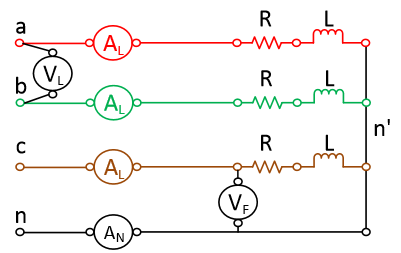
\includegraphics[]{FOTO1.png} 
            \caption{circuito em estrela a ser montado}
            \label{figura:qualquernome}
        \end{figure}
        Para realizar a montagem deve seguir a figura 1, antes de iniciar a montagem certifique-se que o circuito esteja desligado.
        
    \subsubsection{Ligação em Delta}
        \begin{figure}[H]
            \centering % para centralizarmos a figura
            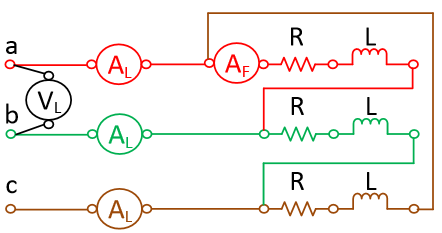
\includegraphics[width=0.8\columnwidth]{FOTO2.png} 
            \caption{circuito em estrela a ser montado}
            \label{figura:montada}
        \end{figure}
        
        
         Para realizar a montagem deve seguir a figura 2, antes de iniciar a montagem certifique-se que o circuito esteja desligado.


\newpage
\section{Análise sobre segurança}
    \mbox{}
    \justifying
    Antes de montar o experimento é importante o uso de equipamentos de proteção, estar com calça, sapatos fechados, sem acessórios metálicos e se o cabelo for grande, este deve estar preso.
    
    A bancada deve estar desenergizada durante a montagem. Durante o experimento não ter contato com nenhum fio ou elemento energizado do circuito além do risco de choque elétrico. Certifique-se de que os equipamentos estão na escala adequada para realizar as medições.
    
    Para movimentar os indutores pegue pela parte inferior evitando riscos de que se desprenda e caia, assim evitando lesões e dano ao dispositivo. 
    
    Realizar as medidas em um tempo curto evitando que o circuito fique energizado por um longo período de tempo, pois os resistores estarão dissipando potência assim esquentando.
    
   Deve-se manter uma distância segura do circuito quando o mesmo está energizado assim evitando queimaduras e choque elétrico.
       

\newpage
\section{Análise}
    \justifying
    \subsection{Dados}
        \subsubsection{Ligação em estrela}
        \justifying
            \begin{table}[H]
         \centering
        \begin{tabular}{|c|c|c|c|c|c|c|c|c|}
              \hline %linha horizontal 
                  fase & V\(_F\)[V] & V\(_L\)[V] & I\(_L\)[A] & I\(_N\)[A] & fp & P[W] & Q[Var] & S[VA] \\
              \hline %linha horizontal 
           a & 56.87 & 99.50 & 0.511 & 0 & 0.565 & 16.43 & 25.00 & 29.06     \\ 
              \hline %linha horizontal 
           b & 58.27 & 100 & 0.495 & 0 & 0.548 & 15.75 & 25.00 & 28.75     \\ 
              \hline %linha horizontal 
           c & 58.34 & 99.6 & 0.553 & 0 & 0.585 & 18.37 & 26.04 & 31.80     \\ 
              \hline %linha horizontal 
           total & - & - & - & - & - & 50.82 & 73.95 & 89.30     \\ 
              \hline %linha horizontal 
        \end{tabular}
        \caption{1Medidas obtidas com neutro conectado (TL = 0000) }
        \end{table}
        
        \begin{table}[H]
             \centering
            \begin{tabular}{|c|c|c|c|c|c|c|c|}
                  \hline %linha horizontal 
                      fase & Vf[V] & V\(_L\)[V] & I\(_L\)[A] & fp & P[W] & Q[Var] & S[VA] \\
                  \hline %linha horizontal 
               a & 56.94 & 99.90 & 0.523 & 0.537 & 15.98 & 25.13 & 29.70     \\ 
                  \hline %linha horizontal 
               b & 58.44 & 101.40 & 0.506 & 0.573 & 16.78 & 24.24 & 29.43     \\ 
                  \hline %linha horizontal 
               c & 58.45 & 99.64 & 0.534 & 0.587 & 18.10 & 25.16 & 30.96     \\ 
                  \hline %linha horizontal 
               total & - & - & - & - & 51.14 & 74.51 & 90.13     \\ 
                  \hline %linha horizontal 
            \end{tabular}
            \caption{Medidas obtidas com neutro desconectado (TL = 0000)}
        \end{table}

    \begin{table}[H]
         \centering
        \begin{tabular}{|c|c|c|c|c|c|}
              \hline %linha horizontal 
                  fase & V\(_L\)[V] & I\(_L\)[A] & P\(_T\)[W] & Q\(_T\)[Var] & S\(_T\)[VA] \\
              \hline %linha horizontal 
           AB & 100.1 & 0.627 & 22.53 & 28.367 & 36.1     \\ 
              \hline %linha horizontal 
           BC & 100.1 & 0.627 & 22.53 & 28.366 & 36.1     \\ 
              \hline %linha horizontal 
           CA & 100.1 & 0.627 & 22.53 & 28.366 & 36.1     \\ 
              \hline %linha horizontal 
           total & - & - & 67.59 & 85.10 & 108.3     \\ 
              \hline %linha horizontal 
        \end{tabular}
        \caption{Medidas obtidas com neutro conectado(TL = 0003)}
    \end{table}

    \begin{table}[H]
         \centering
        \begin{tabular}{|c|c|c|c|c|c|}
              \hline %linha horizontal 
                  fase & V\(_L\)[V] & I\(_L\)[A] & P\(_T\)[W] & Q\(_T\)[Var] & S\(_T\)[VA] \\
              \hline %linha horizontal 
           A & 100.1 & 0.627 & 22.53 & 28.33 & 36.2     \\ 
              \hline %linha horizontal 
           B & 100.1 & - & 22.53 & 28.33 & 36.2     \\ 
              \hline %linha horizontal 
           C & 100.1 & - & 22.53 & 28.33 & 36.2     \\ 
              \hline %linha horizontal 
           total & - & - & 67.59 & 84.99 & 108.6     \\ 
              \hline %linha horizontal 
        \end{tabular}
        \caption{Medidas obtidas com neutro desconectado (TL = 0003) }
    \end{table}





        \subsubsection{Ligação em delta}
        \justifying

    \begin{table}[H]
         \centering
        \begin{tabular}{|c|c|c|c|c|c|c|c|c|}
              \hline %linha horizontal 
                  fase & V\(_L\)[V] & V\(_f\)[V] & I\(_L\)[A] & I\(_f\) & fp & P[W] & Q[Var] & S[VA] \\
              \hline %linha horizontal 
           a & 99.50 & 100.1 & 1.564 & 0.9 & 0.549 & 49.87 & 75.97 & 90.74     \\ 
              \hline %linha horizontal 
           b & 100 & 100.1 & 1.543 & - & 0.556 & 49.30 & 72.60 & 87.46     \\ 
              \hline %linha horizontal 
           c & 99.6 & 100.1 & 1.512 & - & 0.555 & 50.18 & 75.49 & 90.52     \\ 
              \hline %linha horizontal 
           total & - & - & - & - & - & 149.50 & 223.4 & 268.4     \\ 
              \hline %linha horizontal 
        \end{tabular}
        \caption{Medidas obtidas com neutro conectado(TL = 0048)}
    \end{table}
    \begin{table}[H]
         \centering
        \begin{tabular}{|c|c|c|c|c|c|c|c|c|}
              \hline %linha horizontal 
                  fase & V\(_L\)[V] & V\(_f\)[V] & I\(_L\)[A] & I\(_f\) & fp & P[W] & Q[Var] & S[VA] \\
              \hline %linha horizontal 
           a & 101.9 & 100.9 & 1.599 & 0.92 & 0.589 & 52.26 & 78.62 & 95.60     \\ 
              \hline %linha horizontal 
           b & 103.0 & - & 1.670 & - & 0.533 & 50.78 & 75.52 & 92.03     \\ 
              \hline %linha horizontal 
           c & 100.7 & - & 1.607 & - & 0.555 & 52.14 & 78.44 & 95.32     \\ 
              \hline %linha horizontal 
           total & - & - & - & - & - & 155.1 & 237.7 & 282.8     \\ 
              \hline %linha horizontal 
        \end{tabular}
        \caption{Medidas obtidas com neutro desconectado(TL = 0049)}
    \end{table}

        \begin{figure}[h]
            
            \centering % para centralizarmos a figura
           % 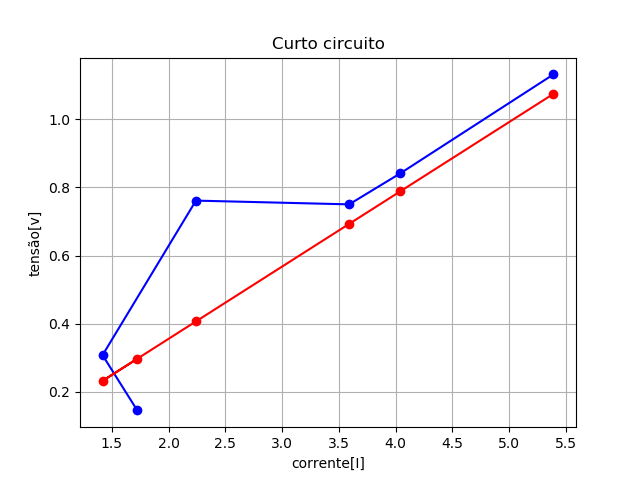
\includegraphics[width=0.8\columnwidth]{Figure_3.png} \\
            \caption{Dados linearizados}
            \label{figura:Dados linearizados}
        \end{figure} 
        
    \subsection{Questões}
        \justifying
        A relação entre V\(_F\) e V\(_L\) da tabela 1 é: \(V_L = \sqrt{3}\times V_F\).
        
        A soma das correntes no neutro foi muito próxima de zero, sendo menor que a precisão do aparelho utilizado o qual indicou 0[A]. Isso ocorre devido ao fato das impedâncias vista pela fonte serem igual e como as tensões aplicadas estão defasadas de \(120^\circ\) a soma é igual a 0.
        
        Se somar fasorialmente as correntes de linhas a soma devera ser iguais a 0 em virtude da Segunda lei de Kirchhoff a qual diz: "a soma das correntes em um nó é igual a zero". Logo \(I_{neutro} = I_{L1}+I_{L2}+I_{L3}\).
         
        Ao interromper a conexão com o neutro as medidas não foram alteradas pela interrupção, os valores foram diferentes pelo fato da tensão disponibilizada pelo varivolt não ser exatamente a mesma que no experimento com neutro conectado. 

        Se desconectasse o neutro e um voltímetro fosse colocado a tensão medida deve ser igual a 0, pois: 
                \[V_F - V_{cargas} = V_N\]
                \[V_F = V_{cargas}\]
                \[V_N = 0\]
    
        A relação \(V_L = \sqrt{3}\times V_F\) para ligaçao em estrela foi comprovada com um erro menor que 1\%. A tabela abaixo mostra o erro entre o valor esperado e o valor medido.
            \begin{table}[H]
         \centering
        \begin{tabular}{|c|c|c|c|c|}
              \hline %linha horizontal 
                  fase & V\(_F\)[V] & V\(_L \)[V](medido) & V\(_L \)[V](esperado) & erro [\%] \\
              \hline %linha horizontal 
           a & 56.87 & 99.50 & 98.50 & 1.01     \\ 
              \hline %linha horizontal 
           b & 58.27 & 100.00 & 100.93 & 0.92     \\ 
              \hline %linha horizontal 
           c & 58.34 & 99.6 & 101.05 & 1.43     \\ 
              \hline %linha horizontal 
        \end{tabular}
        \caption{Relação V\(_L\) e V\(_F\)}
    \end{table}
    
    A relação \(I_L = \sqrt{3}\times I_F\) para ligação em delta foi comprovada com um erro menor que 3\%. A tabela abaixo mostra o erro entre o valor esperado e o valor medido.
    \begin{table}[H]
         \centering
        \begin{tabular}{|c|c|c|c|c|}
              \hline %linha horizontal 
                  fase & I\(_f\) & I\(_L\)[A](medido) & I\(_L\)[A](esperad) & erros [\%] \\
              \hline %linha horizontal 
           a & 0.9 & 1.564 & 1.559 & 0.32     \\ 
              \hline %linha horizontal 
           b & - & 1.543 & 1.559 & 1.03     \\ 
              \hline %linha horizontal 
           c & - & 1.512 & 1.559 & 3.01     \\ 
              \hline %linha horizontal 
        \end{tabular}
        \caption{Medidas obtidas com neutro conectado}
    \end{table}

    Teoricamente as potências deveriam ser as mesmas, contudo os dados não apresentam essa característica. A Tabela abaixo mostra a comparação da potência medida e da potência calculada para encontrar um possível erro cometido durante as medições.


    \begin{table}[H]
         \centering
        \begin{tabular}{|c|c|c|c|c|c|c|c|c|c|}
              \hline %linha horizontal 
                   Ligação & V\(_L\)[V] & I\(_L\)[A] & \(\theta [^\circ]\) & P\(_T\)(medida)[W] & P\(_T\)(calculada)[W] & Q\(_T\)[Var] & Q\(_T\)(calculado)[Var] & S\(_T\)[VA] & S\(_T\)(calculado)[VA] \\
              \hline %linha horizontal 
           estrela & 101.40 & 0.495 & 56.77 & 50.82 & 47.64 & 73.95 & 72.72 & 90.13 & 86.94     \\ 
              \hline %linha horizontal 
           delta & 100 & 1.543 & 56.22 & 149.50 & 148.6 & 223.4 & 222.14 & 268.4 & 267.26     \\ 
              \hline %linha horizontal 
        \end{tabular}
        \caption{Potências calculadas e medidas}
    \end{table}
    As medições foram realizadas corretamente, as potencias foram diferentes pois os circuitos possuem a mesma tensão de Linha (V\(_L\)) porém correntes de Linhas diferente.
    A relação de potências é :  P\(_{delta}  \) = 3\(\times\) P\(_{estrela}\), para transformar um circuito em delta para um equivalente em estrela deve-se dividir as impedâncias por 3. 
    \[Z_{\Delta} = 3\times Z_{Y} \]
    Ao passar a montagem para ligação em delta usou-se as mesmas impedâncias, assim não sendo um equivalente. Isso explica o fato das potencias terem sido diferentes.
    
    As pequenas diferenças entre as tensões e correntes se dão pelo fato de que as impedâncias não possuem exatamente o mesmo valor, vai da construção de cada uma onde são projetadas para admitirem um pequeno erro nos seus valores. Portando se as impedâncias são diferentes então a defasagem das tensões e correntes podem não ficar exatamente 120\(^\circ\) e com isso a corrente no Neutro apresenta um valor diferente de zero.

    Quando o medidor Kron esta configurado para TL = 0003 ele encontra as
    demais medidas com as seguintes expressões as quais são validas para ligação em estrela:
    \[V_{AN} = V_{BN} = V_{CN}\]
    \[V_{AB} = V_{BC} = V_{CA} = \sqrt{3}\times V_{AN}\]
    \[P_T = 3\times V_{AN} \times I_L\times\cos(\theta)\]
    \[Q_T = 3\times V_{AN} \times I_L\times\sin(\theta)\]
    \[S_T = 3\times V_{AN} \times I_L\]
    A vantagem é de com o acesso em uma única fase obter dados do circuito inteiro.
    
    A tensão informada é a tensão de Linha pois \(S = \sqrt{3}\times V_{informado}\times I_L\).
    Deve-se tomar cuidado para não medir tensão de linha no lugar de tensão de fase.
    
    É incorreto pois a corrente no I$_N$ deve ser zero em um circuito equilibrado, assim está não serve para indicar se o circuito está em curto.
    
    Para a corrente em I$_N$ crescer o circuito pode estar em curto com o neutro ou o circuito é desequilibrado(que não é o caso deste experimento) ou o mais provável neste experimento é que uma das fases não estão conectadas assim a corrente em I$_N$ será \(I_1 + I_2\).
\newpage
\section{Simulação}
    \justifying
    Para simulação foi usado o  software Multisim, abaixo a figura do circuito a ser simulado.
  

    \begin{figure}[h]
            \centering % para centralizarmos a figura
          %  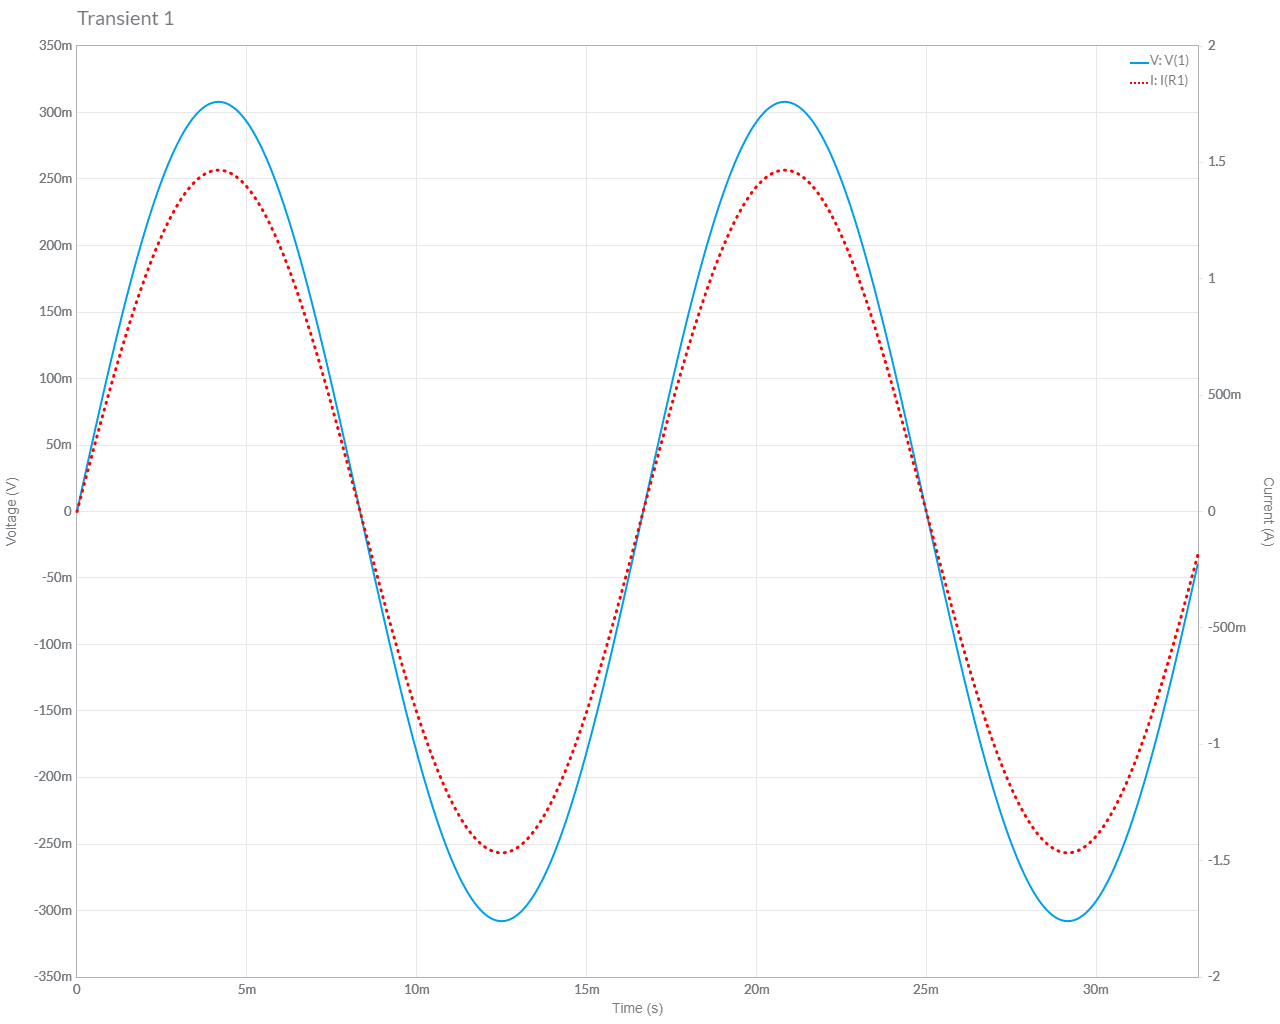
\includegraphics[width=0.8\columnwidth]{Figure_6.png} 
            \caption{Gráfico gerado pelo simulador}
            \label{figura:grafico simulacao}
    \end{figure} 
 
  



    \begin{figure}[H]
            \centering % para centralizarmos a figura
           % 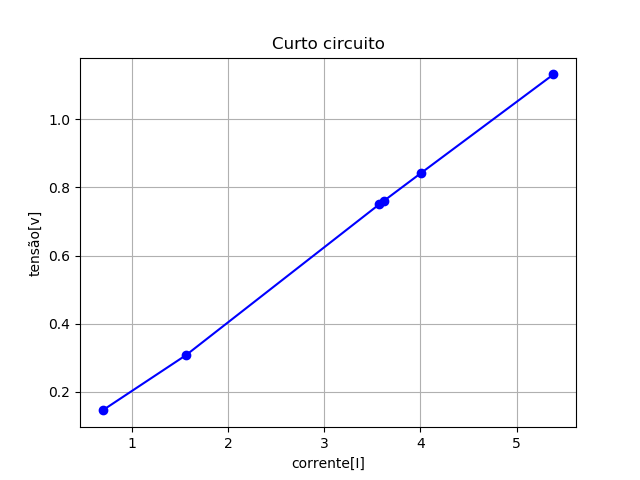
\includegraphics[width=0.8\columnwidth]{Figure_7.png} 
            \caption{Gráfico da tabela 2}
            \label{figura:grafico pontos simulacao}
    \end{figure} 
    Como esperado o gráfico é linear e tem coeficiente \(a = 0.21 \).
        
\newpage
\section{Conclusão}
\justifying
    Foi comprovado neste experimento as relações de tensão e de corrente para circuitos trifásicos equilibrados. Foi visto que a corrente no neutro é praticamente 0[A] devido a soma fasorial das correntes.
    
    Por ser um circuito equilibrado as medições eram para ser as mesmas, porém, além de que é impossível ter uma precisão exata na confecção dos dispositivos existe o erro do aparelho para realizar a medição e a impedância varia com a temperatura do dispositivo.
    
    A simulação apresentou dados ideais e que as medidas eram simétricas, isso acontece pois o software utiliza as equações teóricas e aproximações para determinar os valores. É importante  simular um circuito pois além de confrontar os cálculos analíticos, da uma noção maior do que esperado no circuito.
    
    
\newpage
\section*{Referencias}
\justifying

ALEXANDER, C.K.; SADIKU, M.N. Fundamentos de Circuitos Elétricos. 5ª ed.
Porto Alegre: Mc Graw-Hill, 2015


Multisim https://www.multisim.com/ - simulação


\end{document}



